\documentclass[paper=A4, DIV=10, parskip=half]{scrartcl}

\RequirePackage{hyperref}
\RequirePackage{xcolor}
\hypersetup{%
  colorlinks=false,% hyperlinks will be black
  linkbordercolor=darkgray,% hyperlink borders will be red
  pdfborderstyle={/S/U/W 1}% border style will be underline of width 1pt
}
\RequirePackage{graphicx}

\title{Dog Breed Identification}
\subtitle{Capstone Project Proposal}
\author{Grzegorz Lippe}
\date{\today}

\begin{document}

\maketitle

\section*{Domain Background}

The task of identifying dog breeds is a known topic amongst the community for machine
learning. I've chosen the dog breed identifier amongst the proposed projects, because it
attracted me the most.

The benefit of the dog breed problem is the high availability of labeled datasets which
can be used for training and validation of the model. A quick search on
\href{https://www.kaggle.com/c/dog-breed-identification/notebooks}{kaggle} and
\href{https://github.com/search?q=dog+breed}{github} provide lots of sources.

Also I must admit that it is the most supported task on Udacity's site.

% Student briefly details background information of the domain from which the project is
% proposed. Historical information relevant to the project should be included. It should
% be clear how or why a problem in the domain can or should be solved. Related academic
% research should be appropriately cited. A discussion of the student's personal
% motivation for investigating a particular problem in the domain is encouraged but not
% required. 

\section*{Problem Statement}

The goal of this project is to provide an app, that can take an arbitrary picture and
return a statement of a most likely dog breed. If a picture of a cat or human is provided,
the app should identify the human, but still provide a statement of a most similar looking
dog breed.

% Student clearly describes the problem that is to be solved. The problem is well defined
% and has at least one relevant potential solution. Additionally, the problem is
% quantifiable, measurable, and replicable. 

\section*{Datasets and Inputs}

The data consists of two different sets, provided by Udacity and are described as follows:

\begin{description}
  \item[\href{https://s3-us-west-1.amazonaws.com/udacity-aind/dog-project/dogImages.zip}{dog dataset}]
  The dog data set is already divided into three different datasets (folders)
  for test, training and validation. Each folder contains sub directories of the specific
  formating \texttt{DDD.breed\_name}, where \texttt{DDD} represents a 3 digit number,
  followed by the breed name after a dot. Each subfolder contains a hand full of images of
  the specific breed.
  
  Overall there are 133 different dog breeds, and 835 images provided for validation, 6680
  images for training and 836 images for testing. The images within the training dataset
  are unbalanced, the amount of images per breed varies from 26 for the Norwegian Buhund
  and the Xoloitzcuintli to 77 for the Alaskan Malamute. So some breeds are represented
  roughly 3 times more often.
  
  The dog images contain a singular dog each, mostly of the whole dog, sometimes only of
  the snout, but they are not equally sized, they vary from 5 kB up to 5 MB. Their aspect
  ratios cover all ranges between portrait, landscape and quadratic.
  
  \item[\href{https://s3-us-west-1.amazonaws.com/udacity-aind/dog-project/lfw.zip}{human dataset}]
  The human dataset consists of 13233 images of 5749 persons, which are stored in a
  separate directory named after each  celebrity. The images of the people are already
  cropped and centered around their face and all of the same size of 250x250, but
  the backgrounds vary. Sometimes there are additional people in the background.
\end{description}

% The dataset(s) and/or input(s) to be used in the project are thoroughly described.
% Information such as how the dataset or input is (was) obtained, and the characteristics
% of the dataset or input, should be included. It should be clear how the dataset(s) or
% input(s) will be used in the project and whether their use is appropriate given the
% context of the problem. 

\section*{Solution Statement}

The human face detection will use an \href{https://opencv.org/}{OpenCV} model with a
pre-trained haar cascade dataset of
\href{https://github.com/opencv/opencv/blob/master/data/haarcascades/haarcascade_frontalface_alt.xml}{\texttt{haarcascade\_frontalface\_alt.xml}}
This algorithms provides bounding boxes for each face found in a given image, like shown
in the figure below with an image of Dan Ackroyd:

\begin{center}
  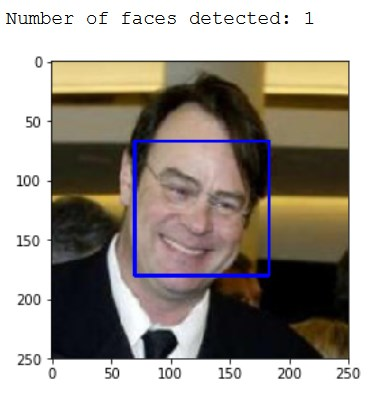
\includegraphics[width=4cm]{images/dan_ackroyd_bounding_box.jpg}
\end{center}

For the dog breed detection a pre trained torch model \texttt{resnet50} is used within a
transfer learning approach. The pre trained model will be trained on the described dog
dataset until it reaches a suitable level of accuracy. The training image data will be
transformed (random resized crop) to a documented
\footnote{\href{https://github.com/pytorch/vision/issues/39}{github.com/pytorch/vision}}
value of 224. Also in the footnote a horizontal flip is performed as an augmentation of
the image. This may be tried as well. 

Since the app shall provide some fun with human images the accuracy of the prediction may
not be that high.

% For the solution a CNN will be build up from scratch. It will involve pre processing the
% data by using torch Transformations:

% \begin{itemize}
%  \item 
% \end{itemize}

% Student clearly describes a solution to the problem. The solution is applicable to the
% project domain and appropriate for the dataset(s) or input(s) given. Additionally, the
% solution is quantifiable, measurable, and replicable. 

\section*{Benchmark Model}

As a benchmark I will use a naive predictor. The dataset is slightly unbalanced so
assuming that there are 133 different dog breeds, some of the occurring up to three times
more than others, the naive approach should guess the correct breed $(b)$ with
$p_{b}=\frac{k_{b}}{3\cdot133}\,,\:k_{b}=\left[1\ldots3\right]$, or less than 1\%. The
implemented model shall get at least 10\%.

% A benchmark model is provided that relates to the domain, problem statement, and
% intended solution. Ideally, the student's benchmark model provides context for existing
% methods or known information in the domain and problem given, which can then be
% objectively compared to the student's solution. The benchmark model is clearly defined
% and measurable.

\section*{Evaluation Metrics}

For the evaluation the labelled data is used. For example the accuracy of the face
detection algorithm can be measured by feeding it with (previously labelled) images of
humans: 

$$ Score = \frac{\textrm{Humans detected}}{\textrm{Images presented}}$$

A slightly modified algorithm can be used to evaluate the dog detecting model. The dog
detector provides a breed identification on top, so in the first step the upper term can
be used to judge the accuracy of the dog detection. Additionally the quality of the breed
identification can be measured as follows:

$$ Score = \sum_{breeds}{\frac{\textrm{correct breed identified}}{\textrm{breed provided}}} $$

% Student proposes at least one evaluation metric that can be used to quantify the
% performance of both the benchmark model and the solution model presented. The evaluation
% metric(s) proposed are appropriate given the context of the data, the problem statement,
% and the intended solution. 

\section*{Project Design}

\subsection*{Main App}

In the initial state the app will consist of a python function which will provide the
following informations: the provided image and a statement of whether a dog or a human
was detected. Additionally a most likely dog breed is provided.
The output may look as follows:

\begin{center}
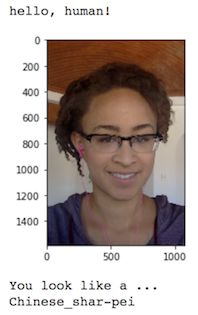
\includegraphics[width=4cm]{images/sample_human_output.jpg}
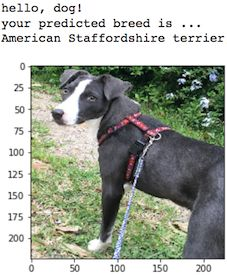
\includegraphics[width=4cm]{images/sample_dog_output.jpg}
\end{center}

In the first iteration the app will fail to provide a reasonable output if some random
"non-dog and non-human" image is provided.

\subsection*{Functions}

The main app above needs two different predictor models to work, a
\texttt{human\_face\_detector} and a \texttt{dog\_breed\_detector}. The two functions are
outlined as follows:

For the \texttt{human\_face\_detector}:

\begin{itemize}
  \item turn the image into grey scale.
  \item use the previously described OpenCV model to detect faces in the given image.
  \item if there are any, proved the bounding boxes for the detected faces.
\end{itemize}

For the \texttt{dog\_breed\_detector}:

\begin{itemize}
  \item load the image into a pyTorch data set, resize (224, 224) and transform to Tensor.
  \item Get the predicted dog breed of the picture.
  \item There will always be a most likely breed. 
\end{itemize}

For the \texttt{main} function:

\begin{enumerate}
  \item Was there any human detected on the image?
  \item If so, provide a statement of a similar looking dog breed.
  \item Are there any dogs on the Image? If so,  provide the most likely breed
\end{enumerate}

% Student summarizes a theoretical workflow for approaching a solution given the problem.
% Discussion is made as to what strategies may be employed, what analysis of the data
% might be required, or which algorithms will be considered. The workflow and discussion
% provided align with the qualities of the project. Small visualizations, pseudocode, or
% diagrams are encouraged but not required. 

% Presentation 

% "Proposal follows a well-organized structure and would be readily understood by
% its intended audience. Each section is written in a clear, concise and specific manner.
% Few grammatical and spelling mistakes are present. All resources used and referenced are
% properly cited."

\end{document}